\documentclass[11pt,twocolumn]{article}

%==============================================================================
% PREAMBLE
%==============================================================================

% Page geometry
\usepackage[letterpaper,margin=0.9in]{geometry}

% Essential packages
\usepackage{amsmath,amssymb,amsfonts}
\usepackage{hyperref}
\usepackage{graphicx}
\usepackage{booktabs}
\usepackage{xcolor}
\usepackage{enumitem}
\usepackage{microtype}
\usepackage{authblk}
\usepackage{listings}
\usepackage{natbib}
\usepackage{tikz}
\usepackage{caption}
\usepackage{subcaption}
\usetikzlibrary{shapes.geometric,arrows.meta,positioning,calc,decorations.pathreplacing}

% Color palette - cohesive and professional
\definecolor{primary}{RGB}{23,63,95}
\definecolor{secondary}{RGB}{60,110,140}
\definecolor{accent}{RGB}{32,178,170}
\definecolor{codebg}{RGB}{248,248,252}
\definecolor{codetext}{RGB}{50,50,70}

% Hyperref setup
\hypersetup{
    colorlinks=true,
    linkcolor=primary,
    filecolor=primary,
    urlcolor=secondary,
    citecolor=secondary,
    pdftitle={SeNARS: Neuro-Symbolic Cognitive Agent},
    pdfauthor={SeNARS Developers}
}

% Code listing style
\lstset{
    basicstyle=\ttfamily\footnotesize\color{codetext},
    keywordstyle=\color{primary}\bfseries,
    commentstyle=\color{secondary}\itshape,
    stringstyle=\color{accent},
    backgroundcolor=\color{codebg},
    breaklines=true,
    frame=single,
    framesep=3pt,
    rulecolor=\color{secondary!30},
    xleftmargin=0.5em,
    xrightmargin=0.5em
}

% Custom commands
\newcommand{\senars}{\textsc{SeNARS}}
\newcommand{\nal}{\textsc{NAL}}
\newcommand{\nars}{\textsc{NARS}}
\newcommand{\tv}[2]{\ensuremath{\langle #1, #2 \rangle}}
\newcommand{\freq}{\ensuremath{f}}
\newcommand{\conf}{\ensuremath{c}}

%==============================================================================
% TITLE
%==============================================================================

\title{\textbf{Semantic Non-Axiomatic Reasoning System (SeNARS):} \\ 
\large A Neuro-Symbolic Cognitive Architecture for Reasoning Under Uncertainty}

\author{SeNARS Developers}
\affil{%
\texttt{senars@narchy.org} \enspace $\bullet$ \enspace 
Matrix: \texttt{\#senars:narchy.org} \enspace $\bullet$ \enspace 
\url{https://github.com/automenta/senars11}%
}

\date{Preprint}

\begin{document}

\maketitle

\begin{center}
\footnotesize
\textit{This work is licensed under Creative Commons Attribution 4.0 International (CC-BY-4.0).} \\
\textit{Source code is released under AGPL-3.0.}
\end{center}

\vspace{0.3em}

%==============================================================================
% ABSTRACT
%==============================================================================
\begin{abstract}
\noindent
\senars{} is a hybrid neuro-symbolic cognitive architecture integrating Non-Axiomatic Logic (\nal{}) with Large Language Models through a streaming pipeline. Beliefs carry explicit uncertainty that revises as evidence accumulates; LLMs contribute pattern recognition and world knowledge. The architecture processes premise streams into conclusion streams, executing symbolic rules synchronously while dispatching neural queries asynchronously.

The prototype implements dual memory, pluggable strategies, and real-time visualization. Yet \senars{} is \emph{deliberately incomplete}: designed as substrate rather than product, it invites diverse forks. This incompleteness is the central innovation---finished systems calcify; open substrates enable ecosystems.
\end{abstract}

%==============================================================================
% 1. INTRODUCTION
%==============================================================================
\section{Introduction}

Artificial intelligence has long been split between two paradigms. \textbf{Symbolic AI} offers transparency: conclusions trace to premises, logical soundness is verifiable, and decisions explain themselves in human terms. But symbolic systems prove brittle when knowledge is incomplete, ambiguous, or contradictory---the everyday condition of intelligent agents navigating uncertain worlds. \textbf{Neural AI}, epitomized by large language models, offers fluid adaptability and astonishing breadth, recognizing patterns across vast corpora and generating plausible responses to almost any prompt. But neural systems hallucinate, lack persistent memory, and cannot explain their reasoning.

Neither paradigm alone suffices for autonomous agents that must reason continuously, learn incrementally, and act reliably under uncertainty.

\subsection{The Neuro-Symbolic Opportunity}

The core insight of neuro-symbolic AI is that these paradigms are \emph{complementary}: symbolic reasoning can constrain and validate neural outputs; neural pattern recognition can inform and accelerate symbolic inference. But effective integration demands more than bolting components together. It requires a coherent architecture where both modalities contribute to a unified reasoning stream.

\senars{} realizes this vision through three architectural commitments:
\begin{enumerate}[itemsep=0.2em,topsep=0.3em]
    \item \textbf{Epistemic Grounding}: All beliefs carry explicit truth values---frequency and confidence---that propagate through inference and revise as evidence accumulates. The system \emph{knows what it knows} and \emph{how much it trusts what it knows}.
    
    \item \textbf{Streaming Dataflow}: Rather than batch processing, \senars{} continuously transforms premise streams into conclusion streams, enabling real-time responsiveness and non-blocking hybrid execution.
    
    \item \textbf{Deliberate Incompleteness}: The architecture provides a stable, extensible core while leaving higher-level decisions open for specialization, enabling diverse forks rather than one-size-fits-all solutions.
\end{enumerate}

\subsection{Vision: An Ecosystem of Minds}

Imagine a future where cognitive architectures are as diverse as biological species. A medical diagnostic system might emphasize caution and explanation; an educational tutor might favor Socratic questioning; a creative assistant might embrace exploratory leaps. All would share common primitives---truth values, memory consolidation, hybrid inference---while diverging in strategy, domain knowledge, and personality.

\senars{} aspires to be the common ancestor: a minimal, coherent substrate from which this ecosystem can evolve. Not a product to be consumed, but a seed to be grown.

%==============================================================================
% 2. BACKGROUND
%==============================================================================
\section{Background}

\subsection{Non-Axiomatic Logic}

\senars{} builds on Pei Wang's foundational work on Non-Axiomatic Logic~\citep{wang2006rigid,wang2013nars}. \nars{} (Non-Axiomatic Reasoning System) was designed for reasoning under the \emph{Assumption of Insufficient Knowledge and Resources} (AIKR)---the premise that any real agent faces incomplete information and limited computation.

Where classical logics require complete, consistent axiom sets, \nal{} operates on partial evidence. Every statement carries a \emph{truth value} comprising frequency (how often true) and confidence (evidential strength). Truth values propagate through inference: conclusions inherit uncertainty from premises, and new evidence revises existing beliefs.

\nal{} is organized into six layers of increasing expressiveness:
\begin{itemize}[itemsep=0.1em,topsep=0.2em,leftmargin=1.2em]
    \item \textbf{NAL-1}: Inheritance relations and basic syllogistic reasoning
    \item \textbf{NAL-2}: Similarity, instances, and properties
    \item \textbf{NAL-3}: Set operations (intersection, union, difference)
    \item \textbf{NAL-4}: Product and image relations
    \item \textbf{NAL-5}: Implication and equivalence (higher-order statements)
    \item \textbf{NAL-6}: Variables, quantification, and temporal reasoning
\end{itemize}

OpenNARS, the reference Java implementation, demonstrated these principles in research settings. ANSNA~\citep{hammer2020ansna} explored a minimal C implementation for embedded systems. \senars{} continues this lineage, reimagining the architecture for modern streaming systems and neural integration.

\subsection{The AIKR Principle}

The \textbf{Assumption of Insufficient Knowledge and Resources} (AIKR) is the foundational premise of \nal{}~\citep{wang2006rigid}. Unlike classical logics that assume complete, consistent knowledge, AIKR acknowledges that any real intelligent agent operates under fundamental constraints:

\begin{description}[style=unboxed,leftmargin=0.5em,itemsep=0.2em]
\item[\textbf{Insufficient Knowledge}] The agent never has complete information about its environment. Facts may be unknown, uncertain, or contradictory. No closed-world assumption is valid.
\item[\textbf{Insufficient Resources}] Computation, memory, and time are always finite. The agent cannot exhaustively explore all possibilities or maintain perfect records.
\item[\textbf{Real-time Demands}] Decisions must be made before complete analysis is possible. Waiting for certainty means missing opportunities.
\end{description}

AIKR has profound implications for system design:

\begin{itemize}[itemsep=0.1em,topsep=0.2em,leftmargin=1.2em]
    \item \textbf{Graded truth}: Beliefs carry explicit uncertainty (frequency and confidence) rather than binary true/false values
    \item \textbf{Evidence accumulation}: New observations revise rather than replace existing beliefs
    \item \textbf{Anytime reasoning}: Inference produces useful partial results at any interruption point
    \item \textbf{Resource-bounded}: Computation is allocated by importance rather than exhaustive search
    \item \textbf{Graceful degradation}: Quality degrades smoothly under resource pressure rather than failing catastrophically
\end{itemize}

\paragraph{How \senars{} Obeys AIKR.} Every architectural decision in \senars{} reflects AIKR:
\begin{itemize}[itemsep=0.1em,topsep=0.2em,leftmargin=1.2em]
    \item \textbf{Truth values} on all beliefs quantify uncertainty explicitly
    \item \textbf{Priority-based sampling} allocates attention to important tasks, not exhaustive search
    \item \textbf{Bounded Focus} limits active working memory, forcing forgetting and consolidation
    \item \textbf{Streaming architecture} produces conclusions continuously rather than in batch
    \item \textbf{Circuit breakers} on LM queries ensure responsiveness under external delays
    \item \textbf{Derivation depth limits} prevent unbounded inference chains
\end{itemize}

The result is a system that remains responsive and useful even when knowledge is incomplete, resources are constrained, and demands are real-time---exactly the conditions that characterize actual intelligent behavior.

\subsection{LLM Reasoning Advances}

Recent work has shown that Large Language Models can approximate structured reasoning when properly prompted:

\textbf{Chain-of-Thought}~\citep{wei2022chain} elicits step-by-step reasoning by including worked examples in prompts, dramatically improving performance on mathematical and logical tasks.

\textbf{ReAct}~\citep{yao2022react} interleaves reasoning traces with actions, enabling LLMs to use external tools and retrieve information mid-reasoning.

\textbf{Reflexion}~\citep{shinn2023reflexion} introduces verbal self-critique: the model reviews its reasoning, identifies errors, and iterates toward better solutions.

\textbf{Toolformer}~\citep{schick2023toolformer} teaches models to invoke APIs (calculators, search engines, databases) by embedding tool calls in training data.

These techniques demonstrate that LLMs can \emph{simulate} structured reasoning. But they lack formal grounding: no explicit uncertainty quantification, no persistent memory across sessions, no guarantee of logical consistency. \senars{} provides the missing infrastructure, using \nal{} as the backbone and LLMs as a knowledge-rich oracle.

%==============================================================================
% 3. ARCHITECTURE
%==============================================================================
\section{Architecture}

\senars{} implements a \textbf{streaming dataflow architecture} that continuously transforms observations and queries into conclusions and actions. The design emphasizes immutability for correctness, non-blocking execution for responsiveness, and explicit extension points for adaptability.

\subsection{Core Data Structures}

All foundational data structures are \textbf{immutable} and \textbf{canonically normalized}, ensuring referential transparency, safe concurrent access, and efficient caching.

\paragraph{Terms.} The fundamental unit of knowledge representation. A Term may be atomic (a symbol like \texttt{bird}) or compound (a relation like \texttt{bird $\rightarrow$ animal}). The \texttt{TermFactory} normalizes equivalent terms---e.g., \texttt{(\&, A, B)} and \texttt{(\&, B, A)} become identical---and caches them for reuse. Each Term carries an operator, complexity measure, and precomputed hash.

\paragraph{Truth Values.} Every statement carries a truth value comprising frequency (how often true) and confidence (evidential strength). Truth values propagate through inference according to \nal{} semantics, ensuring conclusions are never more certain than premises.

\paragraph{Stamps.} Evidence tracking for cyclicity detection, revision, and provenance. Each Stamp records a unique identifier, occurrence time, source (user input, inference, LLM, sensor), and evidential base.

\paragraph{Tasks.} The unit of processing. A Task contains a Term, truth value, stamp, priority, and punctuation indicating its type: \textbf{Belief} (\texttt{.}) for declarative knowledge, \textbf{Goal} (\texttt{!}) for objectives, or \textbf{Question} (\texttt{?}) for queries.

\subsection{The Streaming Pipeline}

\begin{figure}[t]
\centering
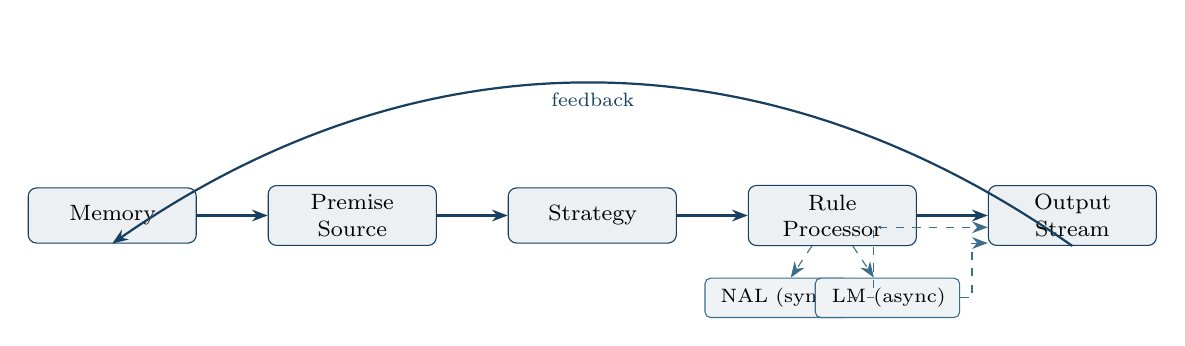
\begin{tikzpicture}[
    node distance=0.6cm and 0.9cm,
    block/.style={rectangle, draw=primary, fill=primary!8, text width=1.9cm, text centered, rounded corners=3pt, minimum height=0.7cm, font=\footnotesize},
    smallblock/.style={rectangle, draw=secondary, fill=secondary!8, text width=1.6cm, text centered, rounded corners=2pt, minimum height=0.5cm, font=\scriptsize},
    arrow/.style={-{Stealth[length=2mm]}, thick, primary},
    dasharrow/.style={-{Stealth[length=2mm]}, dashed, secondary}
]
    % Main pipeline
    \node[block] (memory) {Memory};
    \node[block, right=of memory] (source) {Premise\\Source};
    \node[block, right=of source] (strategy) {Strategy};
    \node[block, right=of strategy] (processor) {Rule\\Processor};
    
    % Rules
    \node[smallblock, below=0.4cm of processor, xshift=-0.7cm] (nal) {NAL (sync)};
    \node[smallblock, below=0.4cm of processor, xshift=0.7cm] (lm) {LM (async)};
    
    % Output
    \node[block, right=of processor] (output) {Output\\Stream};
    
    % Arrows
    \draw[arrow] (memory) -- (source);
    \draw[arrow] (source) -- (strategy);
    \draw[arrow] (strategy) -- (processor);
    \draw[arrow] (processor) -- (output);
    \draw[dasharrow] (processor) -- (nal);
    \draw[dasharrow] (processor) -- (lm);
    \draw[dasharrow] (nal.east) -- ++(0.3,0) |- ([yshift=-0.15cm]output.west);
    \draw[dasharrow] (lm.east) -- ++(0.15,0) |- ([yshift=-0.35cm]output.west);
    
    % Feedback
    \draw[arrow, bend right=35] (output.south) to node[below, font=\scriptsize] {feedback} (memory.south);
    
\end{tikzpicture}
\caption{The \senars{} streaming pipeline. Premises flow from Memory through Strategy and RuleProcessor, producing conclusions that merge into the Output Stream and feed back to Memory.}
\label{fig:pipeline}
\end{figure}

The reasoning engine operates as a continuous pipeline (Figure~\ref{fig:pipeline}):

\begin{description}[style=unboxed,leftmargin=0.5em,itemsep=0.3em]
\item[\textbf{1. PremiseSource}] Samples Tasks from Memory according to configurable objectives:
    \emph{priority} (importance-weighted),
    \emph{recency} (temporal relevance),
    \emph{novelty} (prefer low-derivation-depth tasks),
    \emph{punctuation} (focus on goals or questions),
    \emph{dynamic} (adaptive based on performance).

\item[\textbf{2. Strategy}] Pairs each primary premise with suitable secondary premises for inference. Pluggable implementations:
\begin{itemize}[itemsep=0.1em,topsep=0.2em,leftmargin=1em]
    \item \textbf{BagStrategy}: \nars{}-style priority sampling for anytime reasoning
    \item \textbf{PrologStrategy}: Goal-driven backward chaining with unification
    \item \textbf{ExhaustiveStrategy}: Comprehensive search over related beliefs
    \item \textbf{ResolutionStrategy}: Prolog-like resolution for question answering
\end{itemize}

\item[\textbf{3. RuleProcessor}] Executes inference rules in non-blocking fashion:
\begin{itemize}[itemsep=0.1em,topsep=0.2em,leftmargin=1em]
    \item \textbf{Synchronous NAL rules}: Execute immediately, returning derived Tasks
    \item \textbf{Asynchronous LM rules}: Dispatch without blocking; results merge when ready
\end{itemize}
A \texttt{RuleExecutor} indexes rules by guard conditions, enabling efficient matching through trie-based lookup.

\item[\textbf{4. Output Stream}] Unified stream merging results from both rule types. Consumers (Memory, UI, external systems) receive conclusions as they become available.
\end{description}

\subsection{Inference Rules}

\senars{} implements the full \nal{} rule set across all six layers. Table~\ref{tab:nal-rules} summarizes the core syllogistic rules; the complete implementation includes set operations, higher-order reasoning, and temporal inference.

\begin{table}[t]
\centering
\footnotesize
\caption{Core NAL Syllogistic Rules}
\label{tab:nal-rules}
\begin{tabular}{@{}lll@{}}
\toprule
\textbf{Rule} & \textbf{Premises} & \textbf{Conclusion} \\
\midrule
Deduction & $A \rightarrow B$, $B \rightarrow C$ & $A \rightarrow C$ \\
Induction & $A \rightarrow B$, $A \rightarrow C$ & $C \rightarrow B$ \\
Abduction & $A \rightarrow C$, $B \rightarrow C$ & $A \rightarrow B$ \\
Exemplification & $A \rightarrow B$, $B \rightarrow C$ & $C \rightarrow A$ \\
\midrule
Comparison & $A \rightarrow B$, $A \rightarrow C$ & $B \leftrightarrow C$ \\
Analogy & $A \rightarrow B$, $B \leftrightarrow C$ & $A \rightarrow C$ \\
Resemblance & $A \leftrightarrow B$, $B \leftrightarrow C$ & $A \leftrightarrow C$ \\
\midrule
Revision & Same statement, different evidence & Merged belief \\
\bottomrule
\end{tabular}
\end{table}

Each inference rule has an associated \emph{truth function} that computes the conclusion's truth value from the premises. Table~\ref{tab:truth-funcs} lists the primary truth functions.

\begin{table}[t]
\centering
\footnotesize
\caption{NAL Truth Functions}
\label{tab:truth-funcs}
\begin{tabular}{@{}lp{5.2cm}@{}}
\toprule
\textbf{Function} & \textbf{Application} \\
\midrule
Deduction & Strong forward inference \\
Induction & Generalizing from shared subject \\
Abduction & Hypothesizing shared cause \\
Exemplification & Weak backward inference \\
Comparison & Deriving similarity from common subject \\
Analogy & Transferring via similarity \\
Resemblance & Chaining similarities \\
Revision & Merging independent evidence \\
Negation & Inverting frequency \\
Intersection & Conjunctive combination \\
Union & Disjunctive combination \\
Difference & Set subtraction \\
\bottomrule
\end{tabular}
\end{table}

Language model rules extend symbolic inference with neural pattern recognition. Table~\ref{tab:lm-rules} shows the primary LM integration points.

\begin{table}[t]
\centering
\footnotesize
\caption{Language Model Integration Rules}
\label{tab:lm-rules}
\begin{tabular}{@{}lp{5.2cm}@{}}
\toprule
\textbf{Rule} & \textbf{Function} \\
\midrule
Elaboration & Generate related beliefs from a concept \\
WorldKnowledge & Query factual knowledge to fill gaps \\
Translation & Convert natural language to Narsese \\
Explanation & Generate natural language from derivations \\
Disambiguation & Resolve ambiguous terms using context \\
\bottomrule
\end{tabular}
\end{table}

\subsection{Dual Memory Architecture}

Inspired by cognitive science, \senars{} separates short-term attention from long-term storage:

\paragraph{Focus (Short-term).} A bounded-capacity priority queue holding tasks for immediate processing. The Focus system implements attention: selecting which tasks receive reasoning resources based on priority, recency, and diversity constraints.

\paragraph{Long-term Memory.} Persistent storage for all Concepts (collections of Tasks sharing a common Term). Specialized indexes enable efficient retrieval by relation type (inheritance, implication, similarity).

\paragraph{Consolidation.} Background process that migrates high-value tasks from Focus to long-term storage, and promotes relevant long-term tasks to Focus when attention shifts. Configurable forgetting policies manage memory pressure.

\subsection{Hybrid NAL--LLM Integration}

The key architectural innovation is \textbf{non-blocking hybrid execution}:

\begin{itemize}[itemsep=0.2em,topsep=0.3em]
    \item \textbf{NAL rules} execute synchronously. The complete \nal{}-1 through \nal{}-6 rule set enables inheritance, similarity, conjunction, implication, and temporal reasoning with rigorous truth-value propagation.
    
    \item \textbf{LM rules} execute asynchronously. Queries dispatch to the language model without blocking the main loop; results integrate as they arrive with assigned confidence values reflecting source reliability.
    
    \item \textbf{Circuit breakers} detect LM failures (timeouts, rate limits, errors) and automatically fall back to pure symbolic reasoning, ensuring graceful degradation.
    
    \item \textbf{Validation gates} allow NAL constraints to filter or adjust LM outputs before integration, maintaining epistemic consistency.
\end{itemize}

The result: real-time responsiveness from synchronous symbolic inference, augmented by the knowledge and fluency of large language models when available.

\subsection{The Cognitive Operating System Analogy}

Think of an LLM as a powerful \textbf{ALU} (Arithmetic Logic Unit)---fast at processing symbols but stateless. \senars{} acts as the \textbf{kernel}:
\begin{itemize}[itemsep=0.1em,topsep=0.2em,leftmargin=1.2em]
    \item \textbf{Scheduler}: The Reasoner pipeline determines which ``processes'' get LM time
    \item \textbf{Filesystem}: Memory and Term structures provide persistent state
    \item \textbf{Permissions}: Truth values and stamps determine what information is trusted
    \item \textbf{Goals}: The belief/goal distinction provides intentionality that reactive LLMs lack
\end{itemize}

Where LLMs are fluid and context-dependent, \senars{} provides the \emph{anchor}---stable beliefs that persist across sessions and constrain ephemeral neural outputs.

%==============================================================================
% 4. IMPLEMENTATION
%==============================================================================
\section{Prototype Implementation}

The current \senars{} prototype is implemented in JavaScript (Node.js), chosen for cross-platform portability, web integration, and rapid iteration. The codebase is structured around the architectural components described above.

\subsection{Technology Stack}

\begin{description}[style=unboxed,leftmargin=0.5em,itemsep=0.2em]
\item[\textbf{Core Engine}] Stream-based reasoning pipeline with configurable components (PremiseSource, Strategy, RuleProcessor)
\item[\textbf{Memory System}] Dual-layer architecture (Focus + long-term) with automated consolidation and configurable forgetting policies
\item[\textbf{LM Integration}] Provider registry supporting OpenAI, Anthropic, Ollama, and HuggingFace with automatic failover and circuit breaker protection
\item[\textbf{Parser}] Complete Narsese parser for \nal{} syntax including all operators, truth values, and punctuation
\item[\textbf{Web UI}] React-based visualization for real-time inspection of reasoning traces, concept activation, memory state, and performance metrics
\item[\textbf{Monitoring}] WebSocket-based event streaming for remote observation and debugging
\end{description}

\subsection{Codebase Architecture}

Figure~\ref{fig:codebase} shows the modular structure of the \senars{} implementation: a central core library surrounded by supporting tools and interfaces.

\begin{figure}[t]
\centering
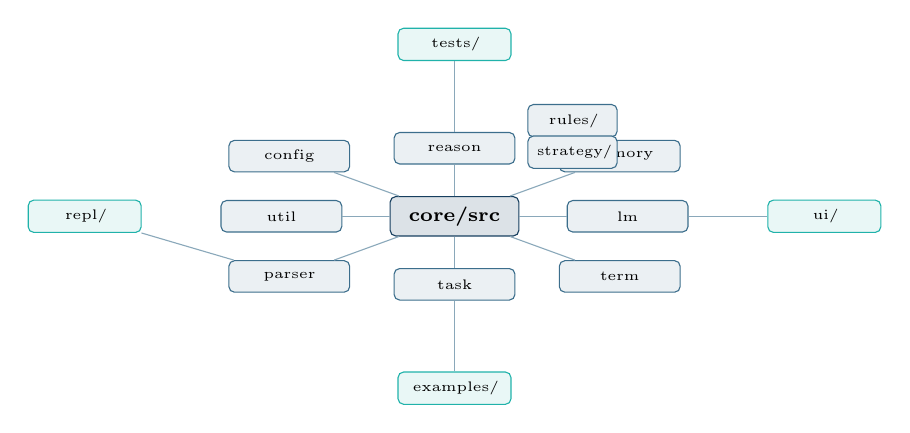
\begin{tikzpicture}[
    node distance=0.5cm,
    core/.style={rectangle, draw=primary, fill=primary!15, text width=1.4cm, text centered, rounded corners=2pt, minimum height=0.5cm, font=\scriptsize\bfseries},
    module/.style={rectangle, draw=secondary, fill=secondary!10, text width=1.3cm, text centered, rounded corners=2pt, minimum height=0.4cm, font=\tiny},
    external/.style={rectangle, draw=accent, fill=accent!10, text width=1.2cm, text centered, rounded corners=2pt, minimum height=0.4cm, font=\tiny},
    conn/.style={-, secondary!60, thin}
]
    % Central core
    \node[core] (core) {core/src};
    
    % Inner ring - core modules
    \node[module, above=0.4cm of core] (reason) {reason};
    \node[module, above right=0.3cm and 0.5cm of core] (memory) {memory};
    \node[module, right=0.6cm of core] (lm) {lm};
    \node[module, below right=0.3cm and 0.5cm of core] (term) {term};
    \node[module, below=0.4cm of core] (task) {task};
    \node[module, below left=0.3cm and 0.5cm of core] (parser) {parser};
    \node[module, left=0.6cm of core] (util) {util};
    \node[module, above left=0.3cm and 0.5cm of core] (config) {config};
    
    % Connections to core
    \foreach \m in {reason,memory,lm,term,task,parser,util,config}
        \draw[conn] (core) -- (\m);
    
    % Outer ring - external interfaces
    \node[external, above=0.9cm of reason] (tests) {tests/};
    \node[external, right=1.0cm of lm] (ui) {ui/};
    \node[external, below=0.9cm of task] (examples) {examples/};
    \node[external, left=1.0cm of util] (repl) {repl/};
    
    % Connections from outer to inner
    \draw[conn] (tests) -- (reason);
    \draw[conn] (ui) -- (lm);
    \draw[conn] (examples) -- (task);
    \draw[conn] (repl) -- (parser);
    
    % Submodules of reason
    \node[module, right=0.15cm of reason, yshift=0.35cm, text width=0.9cm] (rules) {\tiny rules/};
    \node[module, right=0.15cm of reason, yshift=-0.05cm, text width=0.9cm] (strategy) {\tiny strategy/};
    
\end{tikzpicture}
\caption{\senars{} codebase module structure. The core library contains reasoning, memory, language model integration, term/task representations, parsing, and utilities. External interfaces include tests, web UI, examples, and REPL.}
\label{fig:codebase}
\end{figure}

\subsection{Validation}

The prototype includes a comprehensive test suite covering:
\begin{itemize}[itemsep=0.1em,topsep=0.2em,leftmargin=1.2em]
    \item Unit tests for all core data structures (Term, Task, Truth, Stamp)
    \item Integration tests for component interaction
    \item Property-based tests for normalization invariants
    \item End-to-end reasoning chain validation
\end{itemize}

\subsection{Performance Metrics}

Table~\ref{tab:metrics} defines the key performance metrics for evaluating \senars{} deployments. These metrics span reasoning efficiency, memory management, hybrid integration, and system responsiveness.

\begin{table}[t]
\centering
\footnotesize
\caption{Performance Metrics for \senars{} Evaluation}
\label{tab:metrics}
\begin{tabular}{@{}lp{5.5cm}@{}}
\toprule
\textbf{Metric} & \textbf{Relevance} \\
\midrule
\multicolumn{2}{@{}l}{\textit{Reasoning Efficiency}} \\
Inferences/second & Raw symbolic reasoning throughput; measures core engine performance \\
Rule match rate & Fraction of premise pairs yielding valid conclusions; indicates rule coverage \\
Derivation depth & Average chain length; deep chains suggest rich transitive reasoning \\
\midrule
\multicolumn{2}{@{}l}{\textit{Memory Management}} \\
Concept count & Total unique concepts in long-term memory; indicates knowledge breadth \\
Focus utilization & Fraction of Focus capacity actively used; measures attention efficiency \\
Consolidation rate & Tasks migrated per cycle; reflects memory dynamics \\
Cache hit ratio & Term normalization cache effectiveness; reduces redundant computation \\
\midrule
\multicolumn{2}{@{}l}{\textit{Hybrid Integration}} \\
LM query latency & Time from dispatch to result; measures neural responsiveness \\
LM success rate & Fraction of queries returning valid results; indicates reliability \\
Circuit breaker trips & Frequency of fallback activation; measures external service stability \\
\midrule
\multicolumn{2}{@{}l}{\textit{System Responsiveness}} \\
End-to-end latency & Time from input to first output; measures real-time responsiveness \\
Backpressure events & Frequency of pipeline throttling; indicates capacity limits \\
Memory footprint & Peak and steady-state memory usage; constrains deployment targets \\
\bottomrule
\end{tabular}
\end{table}

\subsection{Operational Capabilities}

What works today:
\begin{itemize}[itemsep=0.15em,topsep=0.3em,leftmargin=1.2em]
    \item Complete \nal{}-1 through \nal{}-6 inference with truth propagation
    \item Multiple reasoning strategies (Bag, Prolog, Exhaustive, Resolution)
    \item Configurable sampling (priority, recency, novelty, punctuation, dynamic)
    \item Resource management: CPU throttling, backpressure, derivation depth limits
    \item LM integration with circuit breaker protection
    \item Real-time visualization of reasoning traces
    \item Bidirectional natural language $\leftrightarrow$ Narsese translation
\end{itemize}

\subsection{Example: Transitive Inference}

\begin{lstlisting}[language=,xleftmargin=1em]
Input:  (bird --> animal){0.90, 0.90}.
Input:  (robin --> bird){0.95, 0.90}.

Derived: (robin --> animal){0.855, 0.81}.
  Rule: Deduction
  From: robin-->bird, bird-->animal
\end{lstlisting}

The derived truth value reflects both the frequency and confidence of the premises, reduced through inference to reflect the evidential chain. Conclusions are never more certain than the premises that support them.

\subsection{Example: Knowledge Discovery}

Consider a system learning about a new domain:

\begin{lstlisting}[language=,xleftmargin=1em]
Input:  (salmon --> fish){0.95, 0.90}.
Input:  (fish --> aquatic){0.90, 0.85}.
Input:  (salmon --> pink){0.80, 0.70}.
Query:  (salmon --> ?what)?

Derived: (salmon --> aquatic){0.855, 0.77}.
LM Elaboration: (salmon --> edible){0.85, 0.60}.
LM Elaboration: (salmon --> migratory){0.90, 0.55}.
\end{lstlisting}

The system combines deductive inference (salmon is aquatic) with LM-derived knowledge (salmon is edible, migratory). LM contributions carry lower confidence, reflecting their external source---they can be revised as direct evidence accumulates.

%==============================================================================
% 5. DELIBERATE INCOMPLETENESS
%==============================================================================
\section{Deliberate Incompleteness}

This section articulates the central philosophical and practical innovation of \senars{}: the recognition that \textbf{deliberate incompleteness is a feature, not a bug}.

\subsection{The Calcification Problem}

History shows that ``finished'' systems tend to ossify. Once a platform presents itself as complete, the friction required to modify it increases dramatically:
\begin{itemize}[itemsep=0.15em,topsep=0.2em]
    \item Users depend on specific behaviors
    \item Documentation hardens into dogma
    \item Communities fragment over backward compatibility
    \item Innovation migrates to workarounds rather than foundations
\end{itemize}

Consider the most generative platforms in computing history. Early Unix succeeded precisely because it was \emph{unfinished}---minimal primitives that invited completion. The Linux kernel remains perpetually incomplete, enabling everything from supercomputers to embedded devices. The web browser was deliberately underspecified, spawning an ecosystem of frameworks. Each exemplifies what Gabriel called ``worse is better''~\citep{gabriel1991worse}: simple, incomplete systems that can be completed differently for different purposes.

In AI specifically, the most influential contributions are often frameworks rather than finished products. OpenAI Gym provided minimal abstractions for RL environments. Transformers provided attention mechanisms without prescribing applications. Each enabled diverse completions while preserving a common core.

\subsection{The SeNARS Approach}

\senars{} is explicitly designed as \textbf{substrate rather than product}:

\begin{quote}
\emph{``This is not being built to be a finished application. It is being built to be substrate---the common seed for a future industrial ecosystem of cognitive architectures.''}
\end{quote}

We stabilize the \emph{essential}:
\begin{itemize}[itemsep=0.1em,topsep=0.2em]
    \item The streaming dataflow architecture
    \item The immutable data foundation
    \item The truth-value semantics
    \item The hybrid execution model
\end{itemize}

We deliberately leave open the \emph{contingent}:
\begin{itemize}[itemsep=0.1em,topsep=0.2em]
    \item Optimal memory parameters
    \item Application-specific rule sets
    \item Domain-tailored strategies
    \item Production deployment patterns
\end{itemize}

\subsection{Invitation to Fork}

We envision multiple \senars{} lineages, each completed differently:
\begin{description}[style=unboxed,leftmargin=0.5em,itemsep=0.2em]
\item[\textbf{Minimal Edge Reasoners}] Stripped-down implementations for embedded/IoT applications
\item[\textbf{High-Agency Planners}] Extensions for autonomous goal pursuit and decision-making
\item[\textbf{Educational Sandboxes}] Interactive environments for teaching AI reasoning
\item[\textbf{Personal Memory Layers}] Lifelong persistent context for individual users
\item[\textbf{Multi-Agent Societies}] Distributed reasoning across networks of agents
\item[\textbf{Alternative Logics}] New formal systems building on the stream architecture
\end{description}

All would share the core pipeline, enabling cross-pollination: a performance optimization from one fork could benefit others; a novel strategy could migrate across applications.

\subsection{Explicit Extension Points}

The prototype deliberately exposes these interfaces for specialization:

\begin{description}[style=unboxed,leftmargin=0.5em,itemsep=0.2em]
\item[\textbf{Strategy}] New premise-pairing algorithms can implement the Strategy interface
\item[\textbf{LM Providers}] Custom integrations via the provider registry
\item[\textbf{Memory Policies}] Configurable forgetting, consolidation, and indexing
\item[\textbf{Rule Sets}] Dynamic registration of custom NAL and LM rules
\item[\textbf{Truth Functions}] Alternative uncertainty representations
\item[\textbf{Layers}] Custom connection types (TermLayer, EmbeddingLayer, or novel designs)
\end{description}

\emph{If something you need is not here yet, that is by design. Fork it and grow it into the species you need.}

%==============================================================================
% 6. FUTURE DIRECTIONS
%==============================================================================
\section{Future Directions}

\subsection{Reinforcement Learning from Preferences}

The belief/goal distinction naturally supports \textbf{Reinforcement Learning from Preferences} (RLFP). Rather than hand-crafted reward functions, the system could learn from qualitative comparisons: ``reasoning path A was clearer than path B.'' This enables training discretionary choices---task selection, rule priority, NAL vs.~LM routing---through human feedback on reasoning trajectories.

\subsection{Embodied Grounding}

Formal reasoning about ``fire $\rightarrow$ hot'' differs from \emph{experiencing} heat. Future work might integrate with robotics platforms or simulation environments to ground symbols in sensorimotor experience, enabling perceptual learning and situated reasoning.

\subsection{Lifelong Learning}

Open questions for long-term deployment:
\begin{itemize}[itemsep=0.1em,topsep=0.2em]
    \item How should retention balance against forgetting as knowledge accumulates?
    \item How can new learning integrate without catastrophic interference?
    \item How should the system detect and adapt to distributional shift?
\end{itemize}

\subsection{Scaling Laws}

The relationship between resources and capability in hybrid systems is unexplored. How does reasoning quality scale with memory capacity? With LM size? With rule set complexity? Systematic investigation is needed.

\subsection{Formal Verification}

For safety-critical applications: Can we prove that inferences preserve consistency? Can we bound computation for specific query types? Formal methods could provide guarantees that neither symbolic nor neural systems offer alone.

\subsection{Alternative Implementations}

The architecture is language-agnostic. Future implementations might target:
\begin{itemize}[itemsep=0.1em,topsep=0.2em]
    \item \textbf{Rust}: Performance-critical deployments
    \item \textbf{WebAssembly}: Browser-native execution
    \item \textbf{GPU kernels}: Accelerated embedding-based reasoning
\end{itemize}

\subsection{Call for Collaborators}

We actively invite contributions:
\begin{itemize}[itemsep=0.1em,topsep=0.2em]
    \item Novel reasoning strategies and memory policies
    \item Domain extensions (medicine, law, education, science)
    \item Formal analysis of inference properties
    \item Benchmarking against existing systems
    \item Interface and accessibility improvements
    \item Documentation, tutorials, and educational materials
\end{itemize}

To get started, clone the repository and explore the \texttt{examples/} directory. The Web UI provides immediate visibility into reasoning traces.

%==============================================================================
% 7. CONCLUSION
%==============================================================================
\section{Conclusion}

\senars{} is an experiment in cognitive architecture---and in research methodology.

Technically, it demonstrates that hybrid neuro-symbolic integration can be \emph{streaming}, \emph{non-blocking}, and \emph{epistemically grounded}. The architecture processes continuous premise streams into conclusion streams, executing symbolic rules synchronously while dispatching neural queries asynchronously. Truth values propagate through inference chains. Dual memory balances attention with persistence.

But the deeper contribution is philosophical. By designing \senars{} as incomplete substrate rather than finished product, we aim to \emph{enable} rather than \emph{constrain} the future of neuro-symbolic AI. We stabilize what must be stable (data structures, dataflow, truth semantics) and leave open what should remain contestable (strategies, parameters, applications).

We release \senars{} as a public good. We actively seek collaborators, forks, alternative completions, and entirely new directions we haven't imagined.

\begin{center}
\emph{Fork it, strip it, break it, grow it.} \\
\emph{Build the species you need.}
\end{center}

%==============================================================================
% REFERENCES
%==============================================================================
\bibliographystyle{plainnat}

\begin{thebibliography}{10}

\bibitem[Gabriel(1991)]{gabriel1991worse}
Gabriel, R.~P. (1991).
\newblock The rise of ``worse is better.''
\newblock In \emph{Lisp: Good News, Bad News, How to Win Big}.
\newblock AI Expert.

\bibitem[Hammer \& Lofthouse(2020)]{hammer2020ansna}
Hammer, P. and Lofthouse, T. (2020).
\newblock ANSNA: An attention-driven non-axiomatic semantic navigation architecture.
\newblock In \emph{Artificial General Intelligence Conference (AGI)}.

\bibitem[Schick et~al.(2023)]{schick2023toolformer}
Schick, T., Dwivedi-Yu, J., Dess{\`\i}, R., et~al. (2023).
\newblock Toolformer: Language models can teach themselves to use tools.
\newblock \emph{Advances in Neural Information Processing Systems (NeurIPS)}, 36.

\bibitem[Shinn et~al.(2023)]{shinn2023reflexion}
Shinn, N., Cassano, F., Gopinath, A., Narasimhan, K., and Yao, S. (2023).
\newblock Reflexion: Language agents with verbal reinforcement learning.
\newblock \emph{Advances in Neural Information Processing Systems (NeurIPS)}, 36.

\bibitem[Wang(2006)]{wang2006rigid}
Wang, P. (2006).
\newblock \emph{Rigid Flexibility: The Logic of Intelligence}.
\newblock Springer, Dordrecht.

\bibitem[Wang(2013)]{wang2013nars}
Wang, P. (2013).
\newblock \emph{Non-Axiomatic Logic: A Model of Intelligent Reasoning}.
\newblock World Scientific Publishing.

\bibitem[Wei et~al.(2022)]{wei2022chain}
Wei, J., Wang, X., Schuurmans, D., et~al. (2022).
\newblock Chain-of-thought prompting elicits reasoning in large language models.
\newblock \emph{Advances in Neural Information Processing Systems (NeurIPS)}, 35.

\bibitem[Yao et~al.(2023)]{yao2022react}
Yao, S., Zhao, J., Yu, D., et~al. (2023).
\newblock ReAct: Synergizing reasoning and acting in language models.
\newblock \emph{International Conference on Learning Representations (ICLR)}.

\end{thebibliography}

\end{document}
